%%-----------------------------------------------------------------------
% Loading the packages and classes
%%-----------------------------------------------------------------------

\documentclass[12pt,twoside,a4paper,final]{book}%
\usepackage{a4}%                        %% Verwendet mehr Platz auf einer A4 Seite als Option a4paper in book
\usepackage[english,ngerman]{babel}%    %% Babel Sprachen
\usepackage[latin1]{inputenc}%          %% input encoder f�r umlaute usw.
\usepackage[T1]{fontenc}
\usepackage{amssymb}%                   %% AMS Symbole
\usepackage{amsmath}%                   %% AMS Math Funktionen
\usepackage{amsfonts}%
\usepackage[Sonny]{fncychap}%           %% Chapter Style
\usepackage[english,noprefix]{nomencl}%  %% Nomenclature (Symbolverzeichnis)
\usepackage{makeidx}%                   %% Index
\usepackage{graphicx}%                  %% Graphiken
\graphicspath{{img/}}
\DeclareGraphicsExtensions{.pdf,.jpeg,.png,.jpg}
\usepackage{psfrag}%                    %% Tex-Schriftarten und Formeln in EPS-Grafiken
\usepackage{color}
\usepackage{nicefrac}
\usepackage{ifthen}
\usepackage{fancyhdr}
\usepackage{subfigure}
\usepackage{glossaries}
\usepackage{cite}
\usepackage{listings}
\usepackage{color}
\usepackage[dvipsnames]{xcolor}
\usepackage{rotating}
%Define Acronyms like
% use on every place in your document \gls{mas} for TGM or - for plural - use \glspl for TGMs
% at the first usage of this, the acronym will be introduced, everywhere else it will only be the in the short form: ``Technologisches Gewerbemuseum (TGM)''
% TIPP: USE THIS FOR EVERY NAME/SOFTWARE-TOOL/MAIN PART OF YOUR WORK, like JAVA, - so that, e.g. JAVA is not written Java everywhere else in your thesis.
\newacronym{tgm}{TGM}{Technologischem Gewerbemuseum}
\newacronym{fp}{FP-Analyse}{Function-Point-Analyse}
\newacronym{afa}{AFA}{Abschreibung f�r Abnutzung}

\newacronym{ma}{MA}{Moving Average}
\newacronym{macd}{MACD}{Moving Average Convergence/Divergence}
\newacronym{cci}{CCI}{Commodity Channel Index}
\newacronym{rsi}{RSI}{Relative Strength Indicator}

\newacronym{forex}{FOREX}{Foreign Exchange Market}

\newacronym{bts}{BTS}{Backtesting-Software}
\newacronym{git}{GIT}{GIT-Server}
\newacronym{dde}{DDE}{Dynamic Data Exchange}
\newacronym{ide}{IDE}{Integrated Development Environment}
\newacronym{ib}{IB}{Interactive Brokers}

\newacronym{wcf}{WCF}{Windows Communication Foundation}
\usepackage{multirow}
\usepackage{eurosym}
\usepackage{array}
\usepackage{capt-of}

%%-----------------------------------------------------------------------
% Makro for thick table lines
%%-----------------------------------------------------------------------

\makeatletter
\newcommand{\thickhline}{%
    \noalign {\ifnum 0=`}\fi \hrule height 1.5pt
    \futurelet \reserved@a \@xhline
}
\newcolumntype{"}{@{\hskip\tabcolsep\vrule width 1.5pt\hskip\tabcolsep}}
\makeatother

%%-----------------------------------------------------------------------
% Using the Hyperref-Package for PDF-Online Version
%%-----------------------------------------------------------------------

\def\usehyperref{1}

\ifnum\usehyperref=1
\usepackage[pdftex=true,
  pdftitle={Diplomarbeit},
  pdfauthor={Gottfried Koppensteiner},
  bookmarksopen,
  colorlinks,
  citecolor=blue,
  linkcolor=blue,
  breaklinks%
]{hyperref}%
\fi



%%-----------------------------------------------------------------------
% Rearranging Nomenclature
%%-----------------------------------------------------------------------


\renewcommand{\nomname}{List of symbols}
%\renewcommand{\nompreamble}{The following list only contains symbols
%  that are used continuously throughout the text. Local symbols are
%  not listed.}
\renewcommand{\nomgroup}[1]{
 \ifthenelse{\equal{#1}{A}}{\item[\textbf{General symbols}\bigskip]}{
 \ifthenelse{\equal{#1}{B}}{\item[\bigskip\bigskip\textbf{Chapter 2}\bigskip]}{
 \ifthenelse{\equal{#1}{C}}{\item[\bigskip\bigskip\textbf{Chapter 3}\bigskip]}{
 \ifthenelse{\equal{#1}{D}}{\item[\bigskip\bigskip\textbf{Chapter 4}\bigskip]}{
 \ifthenelse{\equal{#1}{E}}{\item[\bigskip\bigskip\textbf{Chapter 5}\bigskip]}{
 \ifthenelse{\equal{#1}{F}}{\item[\bigskip\bigskip\textbf{Appendix}\bigskip]}{
 }}}}}}}
\makenomenclature



%%-----------------------------------------------------------------------
% Makes Bibliography available in Winedt
%%-----------------------------------------------------------------------

%GATHER{bib_kiefer.bib}


%%-----------------------------------------------------------------------
% Definition of possible environments
%%-----------------------------------------------------------------------

\newtheorem{theorem}{Theorem}[chapter]
\newtheorem{acknowledgement}{Acknowledgement}[chapter]
\newtheorem{algorithm}{Algorithm}[chapter]
\newtheorem{axiom}{Axiom}[chapter]
\newtheorem{case}{Case}[chapter]
\newtheorem{claim}{Claim}[chapter]
\newtheorem{conclusion}{Conclusion}[chapter]
\newtheorem{condition}{Condition}[chapter]
\newtheorem{conjecture}{Conjecture}[chapter]
\newtheorem{corollary}{Corollary}[chapter]
\newtheorem{criterion}{Criterion}[chapter]
\newtheorem{definition}{Definition}[chapter]
\newtheorem{example}{Example}[chapter]
\newtheorem{exercise}{Exercise}[chapter]
\newtheorem{lemma}{Lemma}[chapter]
\newtheorem{notation}{Notation}[chapter]
\newtheorem{problem}{Problem}[chapter]
\newtheorem{proposition}{Proposition}[chapter]
\newtheorem{remark}{Remark}[chapter]
\newtheorem{solution}{Solution}[chapter]
\newtheorem{summary}{Summary}[chapter]
\newenvironment{proof}[1][Proof]{\noindent\textbf{#1.} }{\ \rule{0.5em}{0.5em}}

\renewcommand{\chaptermark}[1]{\markboth{\thechapter.\ #1}{}}
\renewcommand{\sectionmark}[1]{\markright{\thesection.\ #1}}




%%-----------------------------------------------------------------------
% Marking of overfull boxes and increasing of tolerances
%%-----------------------------------------------------------------------

% F�r die Final-Version die n�chste Zeile auskommentieren um schawarze Balken (TU-Logo im Titelblatt) zu ignorieren!
\overfullrule=10pt%                     %% Markiert �berf�llte Boxen. z.b. hbox overfull (Evtl. nicht im pdf sichtbar!!!!)
\hfuzz=1pt%                             %% Toleranz bei hbox overfull erh�ht 1pt entspr. ca. 1/3 mm


%%-----------------------------------------------------------------------
% Counter
%%-----------------------------------------------------------------------


\setcounter{secnumdepth}{3}%
\setcounter{tocdepth}{3}%



% Clear Header Style on the Last Empty Odd pages
\makeatletter
\def\cleardoublepage{\clearpage\if@twoside \ifodd\c@page\else%
    \hbox{}%
    \thispagestyle{empty}%              % Empty header styles
    \newpage%
    \if@twocolumn\hbox{}\newpage\fi\fi\fi}
\makeatother

%%-----------------------------------------------------------------------
% Avoid indents
%%-----------------------------------------------------------------------

\setlength{\parindent}{0pt}

%%-----------------------------------------------------------------------
%% Hyphenation for german abstract
%%-----------------------------------------------------------------------

\hyphenation{Fa-mi-lie
             Ski-bil-dung
             Ar-beits-wal-ze
             neg-lec-ted
             se-par-ate
             di-men-sio-nal
             her-r\"uhren
             N\"a-herungs-l\"os-ungen
             wissen-schaft-licher
             Regelungs-technik
             re-con-fi-gur-abili-ty
             manage-ment
             manu-facturing
             not-wendigen
             }


%%-----------------------------------------------------------------------
% Colored grafix
% 1 = color
% 0 = grey
%%-----------------------------------------------------------------------


\def\colorsw{1}

%%-----------------------------------------------------------------------
% Additional remarks
% 1 = with remarks
% 0 = without remarks
%%-----------------------------------------------------------------------


\def\addnotes{0}


%%-----------------------------------------------------------------------
% Define month
%%-----------------------------------------------------------------------

\def\monthdis{Oktober 2012}

\makeglossaries
%%-----------------------------------------------------------------------
% Document
%%-----------------------------------------------------------------------


\begin{document}%
\selectlanguage{ngerman}%
\renewcommand{\indexname}{Index}%
\topmargin15.0mm


\def\tpdefault{{\sf \center \vspace*{-4cm}
%\begin{center}
%\hspace*{-1.3cm}
%\rule{17cm}{0.02cm}
%\end{center}


\begin{figure}[h]
\begin{flushright}	
		
\includegraphics[width=0.3\textwidth]{graphics/title/tgmlogo2.png}
	\label{fig:tgmlogo}
\end{flushright}
\end{figure}


\vspace{2cm}


{\Large %\bf 
Machbarkeitsstudie\\ \vspace{0.7cm}}
 {\LARGE \sloppy
{\bf \sf  \textbf{AQUILA \\}
Tradingsoftware mit Webschnittstelle
\\}}
%
%
\vspace*{2cm}
{\normalsize Ausgef\"uhrt in Zuge des Projektmanagement-Unterrichts im 5. Jahrgang\\
Ausbildungszweig Systemtechnik/Medientechnik\\ %unzutreffendes streichen
  \vspace{1.5cm}
  \normalsize unter der Leitung von\\
  \large Prof.\ Mag.\ Hans Brabenetz\\
  \normalsize Abteilung f�r
  Informationstechnologie\\
  \vspace{1.5cm}
  eingereicht am  Technologischen Gewerbemuseum Wien\\
  H\"ohere Technische Lehr- und Versuchsanstalt\\
  Wexstrasse 19-23, A-1200 Wien\\
  }}}


\begin{titlepage}
	\tpdefault
	{\sf \center \vspace{1.0cm}
	\normalsize von\\
	\large 
	Peer Nagy 5CHITI\\
	Gabriel Pawlowsky, 5BHITS\\
	Josef Sochovsky, 5BHITS\\
	\vspace {2 cm}
	\bf \sf {Wien, im \monthdis} \\
		%	\vspace{2cm}
	%	\rule{\textwidth}{0.01cm}
	
	}



	\end{titlepage}
\frontmatter%   %% front matter will be numbered in small Roman letters

%%-----------------------------------------------------------------------


%%TCIDATA{OutputFilter=latex2.dll}
%TCIDATA{Version=5.00.0.2552}
%TCIDATA{LaTeXparent=0,0,Dissertation_SW.tex}


\chapter*{Vorwort}

Diese Arbeit wurde im Jahr 2012 im Zuge unserer Ausbildung in der Abteilung f�r Informationstechnologie am \gls{tgm}, HTBLVA Wien 20, durchgef�hrt. 


\bigskip

Dankesworte

\bigskip
\bigskip
\bigskip
\bigskip



Wien, im \monthdis \hfill Name, Name, Name, Name \vfill
%
%\selectlanguage{english}%
%\chapter*{Abstract}

This is the english abstract.%
%\selectlanguage{ngerman}%
%\chapter*{Kurzfassung}

Deutsche Kurzfassung kommt hierher%


%%-----------------------------------------------------------------------
% Define Header for Content chapter
%%-----------------------------------------------------------------------


\makeatletter
\def\tableofcontents{\chapter*{\contentsname\@mkboth{\contentsname}{\contentsname}}
  \@starttoc{toc}}
\makeatother

\clearpage%
\tableofcontents
\clearpage
\listoffigures
\clearpage
\lstlistoflistings %\listoftables
\clearpage 
\markboth{Contents}{Contents}


%\addcontentsline{toc}{chapter}{\numberline{}\listfigurename}%
%\listoffigures
%\listoftables%
%\addcontentsline{toc}{chapter}{\numberline{}\listtablename}%
\clearpage%



\nomenclature[aa]{$t$}{time}
\nomenclature[bb]{$t_0$}{reference time}
\nomenclature[aa]{$m$}{mass}
\nomenclature[aa]{$\rho$}{mass density}

\markboth{\nomname}{\nomname}%
\addcontentsline{toc}{chapter}{\numberline{}\nomname}%
\printnomenclature


\mainmatter%   %% main part will be numbered in Arabic letter


% include chapters
% !TeX root = ../Aquila_Machbarkeitsstudie.tex
% Chapter1

\chapter{Einleitung} \label{chapter:einleitung}

Aktienhandel ist meist mit viel Erfahrung verbunden. Umso kurzfristiger gehandelt wird, desto mehr Konzentration und Aufmerksamkeit muss den Vorg�ngen gewidmet werden, damit auch bei mehreren Trades am Tag summa summarum eine positive Bilanz entsteht. Dies macht es f�r kleine Firmen schwierig und f�r handelnde Privatpersonen nahezu unm�glich in diesem Zeitraum zu operieren. Das Ziel dieses Projektes ist es, genau bei dieser Zielgruppe zu punkten, indem eine Software zur algorithmischen Abbildung eines Handelssystems geschaffen wird, die automatisch Kauf- und Verkaufentscheidungen trifft. Eine Website als Schnittstelle zum Benutzer gew�hrleistet Plattformunabh�ngigkeit, gibt Informationen �ber Performance und Preisentwicklungen und erm�glicht das �ndern von Parametern von �berall. Zus�tzlich k�nnen mehrere Benutzer von unterschiedlichen Standorten mit einem gemeinsamen Portfolio operieren.\\
	Charts auf der Website bieten live einen �berblick �ber die aktuelle Situation und dadurch eine erh�hte Transparenz der Arbeitsweise und Entscheidungsgenerierung des Algorithmus. Relevante Parameter, wie die zu handelnden Aktien oder die H�he der Investition k�nnen ebenfalls einfach �ber die Webschnittstelle ver�ndert werden.%
% !TeX root = ../Aquila_Pflichtenheft.tex

% Chapter2: Produkteinsatz

\chapter{Produkteinsatz} \label{chapter:produkteinsatz}
\section{Anwendungsbereiche und Zielgruppen}

Das Produkt implementiert ein Handelssystem f�r Aktien. Daher ist f�r einen vern�nftigen Umgang mit der Software ein Mindestwissen �ber Aktienhandel und B�rsengesch�fte vorauszusetzen. Vorteilhaft w�re ebenso ein Verst�ndnis von technischer Analyse und h�ufig genutzten Indikatoren, um darauf basierende Handelssysteme zu durchschauen. Programmier- b.z.w. vertiefende Computerkenntnisse m�ssen hingegen nicht vorhanden sein.\\
	Als Zielgruppe sind insbesondere kleine und mittlere Unternehmen (KMU) anvisiert, in denen sich bereits Personen mit finanzwirtschaftlichen Angelegenheiten befassen. Hinzu kommen private Einzelpersonen, die �ber das n�tige Kapital f�r kurzfristigen Aktienhandel verf�gen und mit wenig Aufwand ein Komplettsystem dazu anwenden m�chten.

\section{Betriebsbedingungen}

Die Software soll es prinzipiell erm�glichen unbeaufsichtigt und selbstst�ndig zu arbeiten, wobei, da es sich um einen substanziellen Kapitalaufwand handeln kann, es insbesondere in der Anfangszeit ratsam ist, die Abl�ufe der Software zu �berwachen.\\
	Sowohl die Handelssoftware selbst als auch die Webseite laufen auf einem Server. Beide Komponenten m�ssen die Aufteilung auf und somit die Kommunikation zwischen mehreren Servern nicht unbedingt unterst�tzen, jedoch w�re dies vorteilhaft, da sowohl Zugriffsrechte separat geregelt werden k�nnten, als auch die Handelssoftware die vollen Kapazit�ten des Servers nutzen kann.\\
	Software und Website sollen einen Betrieb rund um die Uhr erm�glichen, ob ein solcher im Einsatz tats�chlich realisiert wird, liegt am Kunden.%
% Chapter3

\chapter{Produktumgebung} \label{chapter:Produktumgebung}

\section{Software}
\label{software}

Um das Ausf�hren der Software zu gew�hrleisten, ist es n�tig einen Webservice anbieten zu k�nnen. Weil das Teilprodukt, die Website, haupts�chlich mit ASP.NET geschrieben ist, muss einer der folgenden Webservern lauff�hig installiert sein:
\begin{itemize}
	\item Internet Information Services (\textbf{IIS})
	\item \textbf{Apache-Webserver} (mit \"mod\_apsdotnet\" und \"mod\_mono\")
	\item \textbf{XSP-Webserver}
	\item \textbf{Cassini-Webserver}
\end{itemize}
Im Falle, dass ein Linuxserver f�r die Website benutzt werden soll wird ein Apache oder der XSP-Webserver empfohlen, damit es zu keinen schwerwiegenden Problemen f�hren kann.
\\
Es wird angeboten die Website und die Software auf unterschiedlichen Computern zu installieren und dort zu benutzen.
F�r das reibungslose Integrieren der Software wird ben�tigt:
\begin{itemize}
	\item Datenbankserver	zum Interagieren mit der Website (Postgresql)
	\item ein installierter und funktionierender \textbf{\gls{ib}-Client}
	\item ein Client von e-Signal
	\item die aktuellste Version des \textbf{.NET-Frameworks}
\end{itemize}

\section{Hardware}
\label{hardware}

Im Falle \textbf{eines} Servers wird ben�tigt der Rechner auf jeden Fall 4 GB Arbeitsspeicher, zirka 100GB freier Speicher und zumindest einen Dual-Core Prozessor.\\
Allerdings liegen diese Werte bereits unter dem heutigen Standard f�r die normalen Server. Wenn man die mindeste Konfiguration w�hlt wird empfohlen keine weiteren Servert�tigkeiten �ber dieses Ger�t zu vollziehen. Es ist au�erdem eine Internetanbindung erforderlich, sowie ausreichend viel Speicherplatz auf der/den Festplatte/n.

\section{Orgware}
\label{orgware}
Der Server, auf dem die Software und die Website verwenden wird, muss mit dem Internet verbunden sein, damit er sich mit \gls{ib}und e-Signal verbinden kann. Dazu wird zuz�glich ein Account dieser beiden Anbieter ben�tigt.%
% Chapter4
\chapter{Produktfunktionen} \label{chapter:thevetestcase}

\begin{quotation}
``The market is not an invention of capitalism. It has existed for centuries. It is an invention of civilization.``
\begin{flushright}
(Mikhail Gorbachev)
\end{flushright}
\end{quotation}%
% Chapter5

\chapter{Wirtschaftliche Machbarkeit} \label{chapter:Wirtschaftliche Machbarkeit}

\section{Aufwandsabsch�tzung}

\begin{figure}[h]
	\centering
		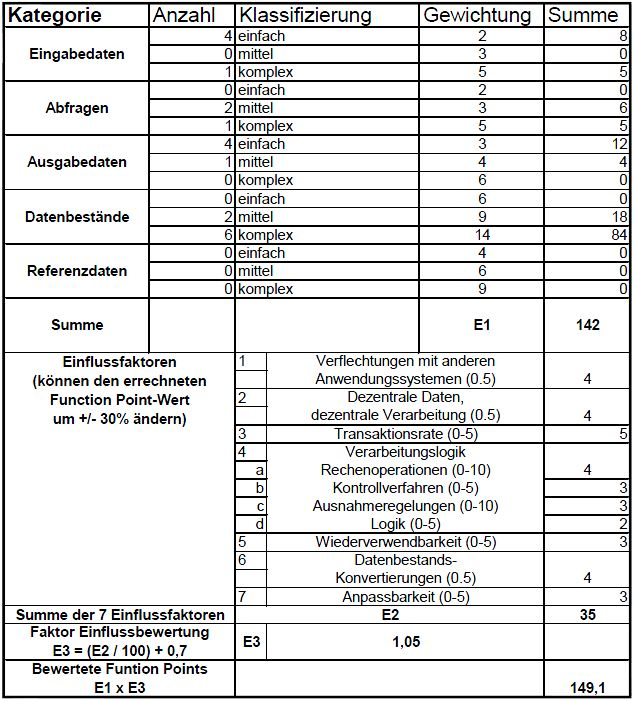
\includegraphics{graphics/chapter5/FunctionPointsAnalysis.JPG}
	\label{fig:FunctionPointsAnalysis}
\end{figure}


\section{Risikoanalyse}
\label{section:Risikoanalyse}

\subsection{Personenausfall}
\label{subsection:Personenausfall}

Eintrittswahrscheinlichkeit:  gering \\
Auswirkungen:  								gering \\

In dem unerwarteten Fall, dass ein Teammitglied l�ngerfristig ausf�llt, muss es m�glich sein die Arbeitsaufgaben dementsprechend neu aufteilen zu k�nnen.
Folgende F�lle k�nnten auftreten:
\begin{itemize}
	\item Streit im Team
	\item Ausfall durch Krankheit oder Tod eines Teammitglieds
	\item Austritt eines Teammitglieds aus dem Projekt
	\item Der Auftraggeber k�nnte aufgrud von Unklarheiten den Projektabbruch initiieren 
	\item Es kann passieren, dass von Seite des Auftragsgebers pl�tzlich kein Interesse an der Umsetzung des Produktes mehr gegeben ist, und es dadurch zu extremem Zeitverzug kommt, was bis zum Abbruch f�hren kann
\end{itemize}

Folgende pr�ventive Ma�nahmen werden eingef�hrt:
\begin{itemize}
	\item Regeln f�r den Umgang innerhalb des Projekts
	\item Ausreichendes Interesse jedes Mitglieds und keine leistungstechnische Probleme 
	\item Gutes Verh�ltnis mit den Auftraggebern
\end{itemize}

\subsection{Zetiliche Risiken}
\label{subsection:Zeitliche Risiken}

Eintrittswahrscheinlichkeit:  gering \\
Auswirkungen:  								mittel \\

Die Aufwands- und Zeitsch�tzung basiert auf dem derzeitigen Lastenheft des Auftraggebers und stellt eine zeitgerechte Fertigstellung sicher. Sollten sich jedoch die Anforderungen des Kunden w�hrend des Projekts �ndern, so wird sich das mit gro�er Wahrscheinlichkeit verz�gernd auf den Fertigstellungstermin auswirken. Die mit dem Kunden vereinbarte Funktionsanalyse und die Meilensteine mit gemeinsam festgelegten Qualit�tskriterien sollten jedoch diesem Risiko entgegenwirken.

\subsection{Technische Risiken}
\label{subsection:Technische Risiken}
\textbf{Datenverlust}\\
Eintrittswahrscheinlichkeit:  gering \\
Auswirkungen:  								mittel \\

Aufgrund der nicht auszuschlie�enden Gefahr des Datenverlusts, muss daf�r gesorgt werden die Sicherheit der Daten, sowie auch die Verf�gbarkeit dieser zu garantieren. Dieses Problem wird mithilfe eines \gls{git} gel��t, durch diesen Server ist es m�glich die Versionen der Software immer zug�nglich zu machen und zus�tzlich die Daten auf den Computern der Projektmitgliedern zu speichern.


\section{Kosten / Nutzenpotential}

* Was k�nnte an Umsatz entstehen?
* Lizensierung des Gesamtpaketes	->	Softwareverkauf + Installation der Webseite
* Kosten aus FP-Analyse gegenrechnen

Das Ziel des Projektes Aquila ist es einerseits eine Variante zur Automatisierung des Aktienhandels zu schaffen und dabei die volle Kontrolle und �bersicht zu behalten. Andererseits liegt ein langfristiger Nutzen in der Entstehung von Knows-How und der technischen Fortbildung des Projektteams; schlie�lich ist das Kapital Bildung bei der Abw�gung des Nutzens nicht au�er Acht zu lassen.\\
Die Tradingsoftware samt Website zur Steuerung dieser soll als einfach zu bediendes Komplettpaket angeboten werden. Die Nutzungs- und Vertriebsrechte bleiben bei den Entwicklern, verkauft werden k�nnen Lizenzen mit beliebig beschr�nkter Nutzerzahl zu unterschiedlichen Preisen.\\
*zB: Einzellizenz, 5-Benutzer, Unlimited
Ebenfalls in Rechnung gestellt wird die Installation der Software auf einem entweder bereits verf�gbaren System oder es wird die ben�tigte Serverarchitektur gemietet. Das Service der Serverbereitstellung ist von Auftragnehmerseite nicht vorgesehen. Sollte dies allenfalls gew�nscht werden, wird das Hosting vermutlich outsourced gemanaged.\\
Die Trading-Software trifft vollst�ndig automatisiert Entscheidungen zum Kauf und Verkauf von Wertpapieren und erm�glicht es somit auch potentiellen Marktteilnehmern mit wenig Zeit systemisch zu handeln, was ohne Software mit erheblichem Zeitaufwand einhergeht. Die Software bleibt dabei ebenfalls stets ver�nder- und erweiterbar; Kunden k�nnten zuk�nftige, neue Softwareversionen gegen Abopreis verrechnet, beim Initialkaufpreis einberechnet oder einzeln verkauft werden. Die Website erm�glicht das gesamte Controlling der Software und bietet neben Konfiguration der Handelseigenschaften �berblick �ber aktuelle Vorg�nge. \\
Die Software ist auf das Handeln �ber einen Broker-Account ausgelegt, wodurch eine Zielgruppe von privaten oder institutionellen Einzeltradern oder kleinen Tradinggruppen angesprochen werdeb. Ebendiese Zielgruppe profitiert besonder von der Simplizit�t der Verwaltung, der �bersicht und des Erweiterungs- und Verbesserungspotentials.%
\chapter{Produktleistungen} \label{chapter:Produktleistungen}

%
\chapter{Management Summary} \label{chapter:management_summary}

Nach ausf�hrlicher Besch�ftigung mit den kritischen Themen sind f�r das Projekt AQUILA geeignete L�sungswege entwickelt worden und es wurde aus mehreren potentiellen Varianten die g�nstigste ausgew�hlt. Folglich ist das Projekt durchf�hrbar.\\
\\
Aus der Variantenbildung ergab sich die Wahl der Programmiersprachenkombination C\#/F\# f�r die Software, da dadurch die Performance der Programmierung und der Ausf�hrung gleicherma�en gegeben ist. Die Webschnittstelle soll in ASP.NET implementiert werden, da dadurch die Funktionen der .NET-API weitergehend verwendet werden k�nnen. Weil beide Technologien aus einer Hand kommen, kann \gls{wcf} f�r die Schnittstelle zwischen beiden Komponenten verwendet werden.\\
\\
Die Gesamtkosten des Projektes wurden auf \EUR{44381} veranschlagt. Empfohlene Preise f�r die Software liegen bei \EUR{1999} f�r eine Einzelbenutzerlizenz, \EUR{4999} f�r eine 5-Benuter Lizenz und \EUR{9999} f�r eine unbeschr�nkte Lizenz.\\
\\
Der gesch�tzte Aufwand des Projektes betr�gt 213.3 Stunden, der auf 3 Projektteammitglieder aufgeteilt wird. Der geplante Projektzeitraum ist vom 14.11.2012 bis 10.04.2013.
%
\chapter{Qualit�tsbestimmung}
\label{chapter:Qualit�tsbetimmung}

\begin{center}

\begin{tabular}{ | l  c  c  c  c |}
\hline 
\textbf{Produktqualit�ten}�& \textbf{Sehr Gut} & \textbf{Gut} & \textbf{Normal} & \textbf{Nicht relevant}\\  \hline
\textbf{Funktionalit�t} & X & & & \\
Angemessenheit & X & & & \\
Richtigkeit & X & & & \\
Interoperabilit�t & X & & & \\ 
Ordnungsm��igkeit & X & & & \\
Sicherheit & & X & & \\
\textbf{Zuverl�ssigkeit} & & X & & \\
Reife & & & X & \\
Fehlertoleranz & & X & & \\
Wiederherstellbarkeit & X & & & \\
\textbf{Benutzbarkeit} & & X & & \\
Verst�ndlichkeit & & X & & \\
Erlernbarkeit & & & X & \\
Bedienbarkeit & X & & & \\
\textbf{Effizienz} & X & & & \\
Zeitverhalten & & X & &  \\
Verbrauchsverhalten & X & & & \\
\textbf{�nderbarkeit} & & X & & \\
Analysierbarkeit & X & & & \\
Modifizierbarkeit & & X & & \\
Stabilit�t & X & & & \\
Pr�fbarkeit & X & & & \\
\textbf{�bertragbarkeit} & & & X & \\
Anpassbarkeit & & X & & \\
Installierbarkeit & & & X & \\
Konformit�t & & & X & \\
Austauschbarkeit & & & X & \\ \hline
\end{tabular}
\end{center}

\newpage
\textbf{Funktionalit�t}
\\
\\
Es ist notwendig, dass die Funktionalit�t des Produkts sehr zuverl�ssig ist. Bei einem Versagen kann es schnell zu einem sehr gro�en Kapitalverlust kommen. Dies ist nat�rlich der Worst-Case. Allerdings m�chte man mit diesem Produkt eine allzeitbereite Plattform anbieten, der man vertrauen kann und auf keinen Fall ein Produkt, das schnell vom Konsumenten abgetan wird, weil es nicht zuverl�ssig arbeitet. \\
Es ist wichtig, dass die Daten, die gespeichert/ausgegeben/mitgeloggt werden, immer der Richtigkeit entsprechen und nicht falsch sind. Diese Daten unterliegen einer Ordnung, die immer die gleiche sein und keine willk�rlichen �nderungen beinhalten soll. \\
Nat�rlich ist die Sicherheit auch ein wichtiges Thema, denn wenn darauf zu wenig geachtet wird, kann unerlaubtes Personal oder Au�enstehende zu viel Einsicht in Firmenangelegenheiten erhalten; Dann kann auch passieren, dass unerlaubte �nderungen am Verhalten der Software vorgenommen werden.
\\
\\
\textbf{Zuverl�ssigkeit}
\\
\\
Das entwickelte Produkt soll zuverl�ssig arbeiten und keine Abst�rze verzeichnen. Es hat einen wohl �berlegten Grundgedanken und wandelt diesen um. Die Entscheidungen, die es trifft, basieren immer nur auf den Einstellungen des Benutzers und werden nicht willk�rlich oder ohne logische Begr�ndung getroffen.\\
Die Fehlertoleranz soll es erm�glichen, bei einer fehlerhaften Daten�bertragung kein Programmversagen zu verursachen. \\Falls es doch zu einem Absturz kommt, kann mittels der Logs und den gespeicherten Transaktionen in der Datenbank das Produkt vollst�ndig wiederhergestellt werden.
\\
\\
\textbf{Benutzbarkeit}
\\
\\
Die Benutzbarkeit ist ein wichtiges Thema, welches auf keinen Fall au�er Acht gelassen werden darf. Die Absicht des Trading ist komplex genug, deswegen soll sich der Benutzer nicht noch zus�tzlich mit einem komplexen und �berladenen Produkt �berfordert f�hlen. Es soll leicht verst�ndlich sein und man soll kein neues Wissen erlernen m�ssen, um damit umzugehen. Die Bedienung soll schnell und effizient von der Hand gehen und den Benutzer nicht allzu viel Zeit kosten.
\\
\\
\textbf{Effizienz}
\\
\\
Es ist wichtig, dass das Handeln mit Wertpapieren schnell vonstatten geht und den Computer nicht �berm��ig belastet. Bei zu gro�er Rechenzeit kann es passieren, dass der berechnete Wert nicht mehr f�r das gegenw�rtige Zeitfenster passt\.\
\\
\textbf{�nderbarkeit}
\\
\\
Bei diesem Produkt ist es sehr wichtig, die Ergebnisse analysieren zu k�nnen. An dem Erzeugnis selbst soll man nicht mehr viel �ndern.
\\
\\
\textbf{�bertragbarkeit}
\\
\\ 
Das Produkt wird vom Projektteam auf eine Kundenumgebung portiert, aber danach ist es f�r das Projekt nicht relevant, weitere Leistungen diesbez�glich anzubieten.%
\chapter{Globale Testf�lle}
\label{chapter:Globale_Testf�lle}

/T010/ \textbf{Angabe eines falschen Accounts} \\
Wenn ein Benutzer auf der Website versucht sich mit einem nicht vorhandenen Benutzernamen oder einem falschen Passwort anzumelden soll es ihm nicht m�glich sein, weitere Einstellungen oder Ver�nderungen am System vorzunehmen.
\\ \\
/T020/ \textbf{B�rse hat geschlossen} \\
Wenn dieser Fall eintritt soll weiterhin die M�glichkeit bestehen, auf der Website Einstellungen und Ver�nderungen vorzunehmen, wenn diese die Software betreffen, wird diese, diese �nderungen �bernehmen und bei Ablaufstart anwenden.
\\ \\
/T040/ \textbf{Aktie entfernen}\\
Eine Aktie, mit der gehandelt wird, soll einfach und schnell �ber die Website aus dem Handelumfang der Software entfernt werden k�nnen. Es ist wichtig, dass diese Funktion sehr schnell abl�uft, damit die zu entfernende Aktie nicht l�nger gehandelt wird.
\\ \\
/T040/ \textbf{Empfangen der Einstellungen von der Website} \\
Wenn die Website Befehle erh�lt, die Einstellungen der Software zu �ndern sollen diese �nderungen an die Software �bertragen  und dann �bernommen werden. Dies soll im Logfile ersichtlich sein.
\\ \\
/T050/ \textbf{Aktie hinzuf�gen} \\
Es soll auf der Website m�glich sein, eine Aktie mit der gehandelt werden soll hinzuzuf�gen. Diese Einstellung soll �ber die Verbindung mit Software direkt �bergeben werden und sofort in Kraft treten. Diese Interaktion ist essentiell, weil man nicht mit langen Wartezeiten rechnen soll, bevor eine neue Aktie hinzugef�gt werden kann.
\\ \\
/T060/ \textbf{Daten empfangen, Log bearbeiten und Entscheidung speichern} \\
Nach dem Start der Software sollen Daten empfangen werden, diese Daten werden dann in den Algorithmus eingespeist um mit ihnen zu rechnen. Das Ergebnis dieses Prozesses ist eine Entscheidung. Diese kann man im Log, in der Datenbank oder auch auf der Website nachvollziehen.
\\ \\
/T070/ \textbf{Charts anzeigen} \\
Auf der Website soll es m�glich sein Charts zu den aktuellen Berechnungen zu sehen, zus�tzlich kann man auf der gleichen Seite auf der sich die Charts befinden, auch die letzte Entscheidung des Algorithmus betrachten. Dadurch erkennt man die Konnektivit�t zwischen Website und Software.%
\chapter{Entwicklungsumgebung}
\label{chapter:Entwicklungsumgebung}%
% Vertragsgegenstand nicht einbinden
%\chapter{Vertragsgegenstand}
\label{chapter:Vertragsgegenstand}

Das Produkt Aquila besteht aus der Software, der Website und der Datenbank zur Verbindung der beiden. Alle diese Teilprodukte werden auf eine DVD gebrannt und in dieser Form an den Kunden �bergeben.\\
\\
Dies Software soll dabei einerseits also portable Version (ausf�hrbare .exe-Datei) und andereseits als Setup-Version zur Installation am Rechner des Kunden vorhanden sein. Zus�tzlich wird ein Benutzerhandbuch mitgeliefert, dass den generellen Umgang mit der Software und ihre Verbindung zur Datenbank beschreibt.\\
\\
Die Datenbank wird in Form eines CreateScripts geliefert, mit dem der Kunde das Datenbankschema in seinen eigenen Datenbankserver integrieren kann. Hierzu wird ebenfalls eine Anleitung geliefert, die diesen Vorgang beschreibt.\\
\\
Die Website wird einfach in Form einen Ordners mit allen ben�tigten Dateien auf der endg�ltigen DVD vorhanden sein. Dieser wird auch eine Anleitung beigelegt, die das aufsetzen der Website beschreibt, sofern schon eine funktionierende Konfiguration von einem der unterst�tzen Webserver vorliegt.\\
\\
Allgemein ist zu sagen, dass das Komplettpaket Aquila in einem Lizenzmodell vertrieben wird, die Eigentumsrechte jedoch bei den Erzeugern bleiben.%
% !TeX root = ../Aquila_Pflichtenheft.tex

\chapter{Projektplanung} \label{chapter:Projektplanung}
\section{Projektstrukturplan}

{\centering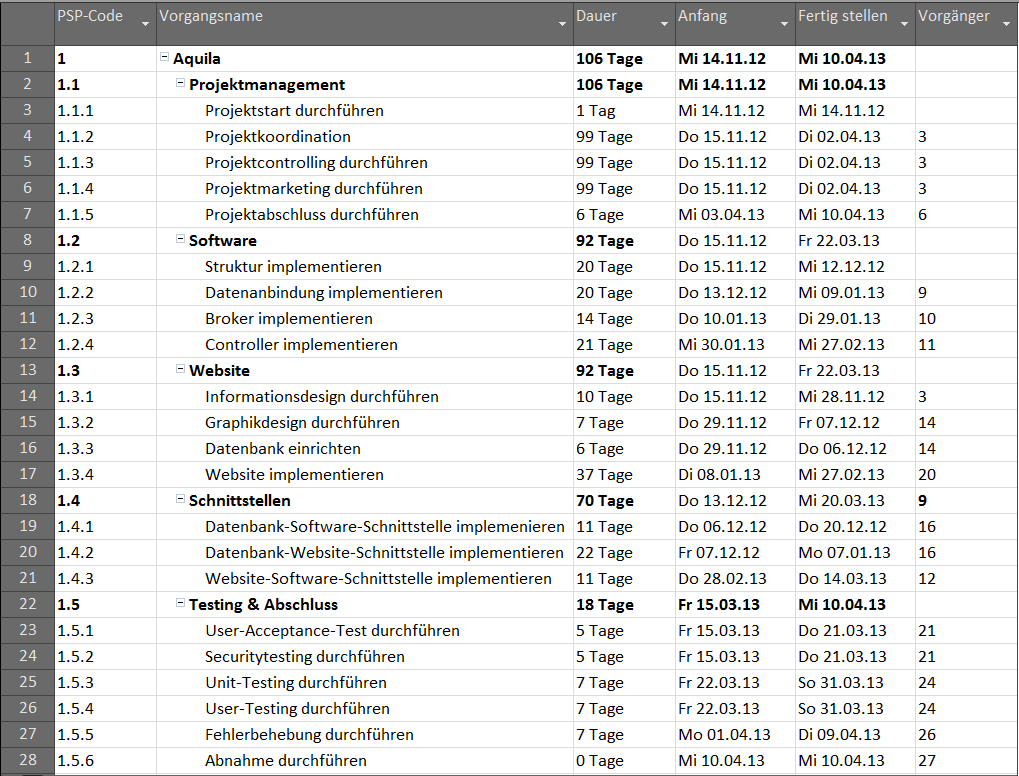
\includegraphics[width=1.00\textwidth]{graphics/projektplanung/psp.png}
\captionof{figure}{Projektstrukturplan}}

\section{Balkenplan}

{\centering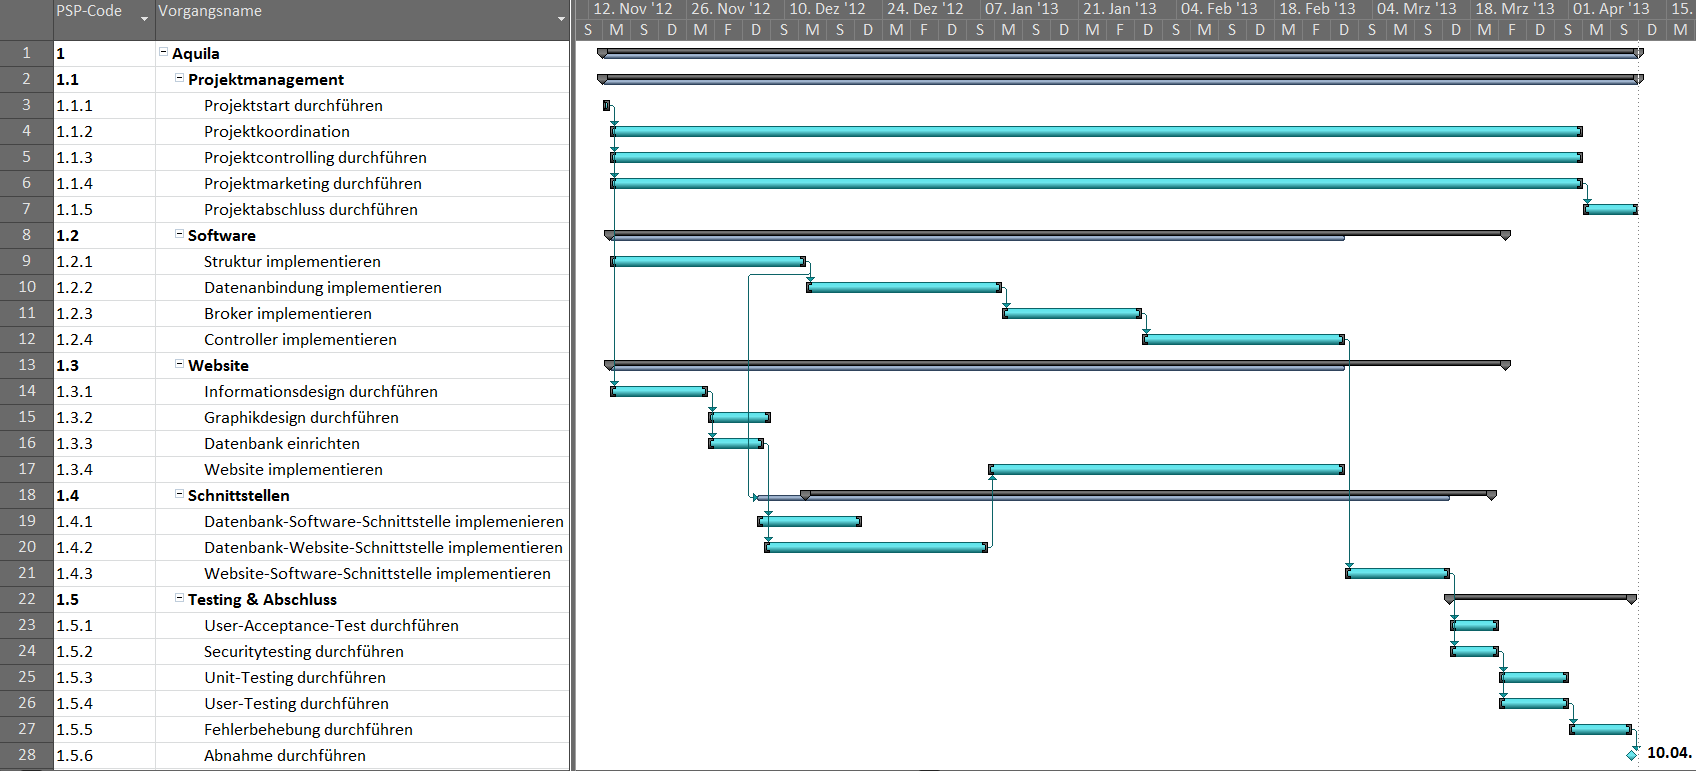
\includegraphics[width=1.00\textwidth]{graphics/projektplanung/balkenplan.png}
\captionof{figure}{Balkenplan}}

\section{Meilensteinplan}

\begin{center}

\begin{tabular}{ | p{3.5cm} | p{7.5cm} | l |}
\hline 
\textbf{Meilenstein} & \textbf{Deliverable} & \textbf{Datum}\\  \hline
Projektstart & ~ & 14.11.2012 \\  \hline
Datenbank eingerichtet & Script zum Erstellen der Datenbank + dazugeh�rige Dokumentation & 06.12.2012 \\ \hline
Externe Schnittstellen implementiert & Schnittstellen zur Kommunikation mit eSignal und InteractiveBrokers + dazugeh�rige Dokumentation & 29.01.2013 \\ \hline
Software \& Website fertiggestellt & Tradingsoftware mit simplem Algorithmus und Websiteoberfl�che und Charting + dazugeh�rige Dokumentation & 27.02.2013 \\ \hline
Produkt fertiggestellt & Version des Produkts (inklusive aller internen Schnittstellen), die noch nicht getestet wurde und ihre Dokumentation & 14.03.2013 \\ \hline
Testing abgeschlossen & Testberichte und etwaige Verbesserungen am Produkt & 09.04.2013 \\ \hline
Projektabnahme & Ausgef�lltes Abnahmeprotokoll & 10.04.2013 \\ \hline

\end{tabular}

\end{center}%
\chapter{Termine}
\label{chapter:Termine}

%
% !TeX root = ../Aquila_Pflichtenheft.tex

\chapter{Versionierung} \label{chapter:versionierung}
\begin{center}

\begin{tabular}{ | l | p{2cm} | p{2cm} | p{2cm} | p{1.5cm} | p{2.8cm} | }
\hline 
\textbf{Version} & \textbf{Autor} & \textbf{QS} & \textbf{Datum} & \textbf{Status} & \textbf{Kommentar} \\  \hline
0.1 & Nagy & & 25.10.2012 & draft & Ziel\-bestimmungen \\ \hline
0.2 & Pawlowsky & Sochovsky & 31.10.2012 & draft & Produkt\-funktionen, Produkt\-daten, Entwick\-lumgsumgebung \\ \hline
0.3 & Nagy & & 31.10.2012 & draft & Ziel\-bestimmungen, Produkteinsatz \\ \hline
0.4 & Nagy & & 01.11.2012 & draft & Produkt\-leistungen \\ \hline
0.5 & Sochovsky & Nagy & 02.11.2012 & draft & Produkt\-umgebung, Globale Testf�lle Qualit�ts\-bestimmungen \\ \hline
0.6 & Nagy & & 04.11.2012 & draft & Benutzer\-schnittstelle \\ \hline
\end{tabular}

\end{center}%




\addcontentsline{toc}{chapter}{Glossary} 
%\printglossary[type=\acronymtype]

%\printglossary[type=\acronymtype]
%\printglossary[type=\acronymtype,style=listwithwidth]

%% include appendix
\begin{appendix}
\printglossary[type=\acronymtype]
\end{appendix}

% Use of the sorted IEEE style, with changes:
% "dashification" was disabled


\cleardoublepage

% IEEE Style
\bibliographystyle{sty/IEEEtranS}

% GATHER
%\input "bib_file.bib"
\phantomsection{}
\addcontentsline{toc}{chapter}{\bibname}
\pagestyle{myheadings}\markboth{\bibname}{\bibname}
\bibliography{tex/bib_file}

%%% generate index
%\clearpage%
%\markboth{\indexname}{\indexname}%
%\printindex%
%\addcontentsline{toc}{chapter}{\numberline{}\indexname}%

%% include affidavit
\thispagestyle{empty}
\vspace*{2cm}
\begin{center}
{\bf \sf \huge Erkl{\"a}rung}
\end{center}
{\sf \vspace{1cm} Hiermit erkl{\"a}ren wir, dass die vorliegende
Arbeit ohne unzul{\"a}ssige Hilfe Dritter und ohne Benutzung
anderer als der angegebenen Hilfsmittel angefertigt wurde. Die aus
anderen Quellen oder indirekt �bernommenen Daten und Konzepte sind
unter Angabe der Quelle gekennzeichnet.

Die Arbeit wurde bisher weder im In- noch im Ausland in gleicher
oder in {\"a}hnlicher Form in anderen Pr{\"u}fungsverfahren
vorgelegt.
\\[1.5cm]
Wien, im \monthdis
\\[2cm]
Name1
\\[2cm]
Name2
\\[2cm]
Name3
\\[2cm]
Name4
\\[2cm]
}%end sf
%



\end{document}
%%%%%%%%%%%%%%%%%%%%%%%%%%%%%%%%%%%%%%%%%%%%%%%%%%%%%%%%%%%%%%%%%%%%%%%%%%%%%%%%%%%%%%%%%%%%%%%%%%%
%%%%%%%%%%%%%%%%%%%%%%%%%%%%%%%%%%%%%%%%%% End Dokument %%%%%%%%%%%%%%%%%%%%%%%%%%%%%%%%%%%%%%%%%%%
%%%%%%%%%%%%%%%%%%%%%%%%%%%%%%%%%%%%%%%%%%%%%%%%%%%%%%%%%%%%%%%%%%%%%%%%%%%%%%%%%%%%%%%%%%%%%%%%%%%
